\section{Intersections Between
Features}\label{intersections-between-features}

\begin{figure}[htbp]
\centering
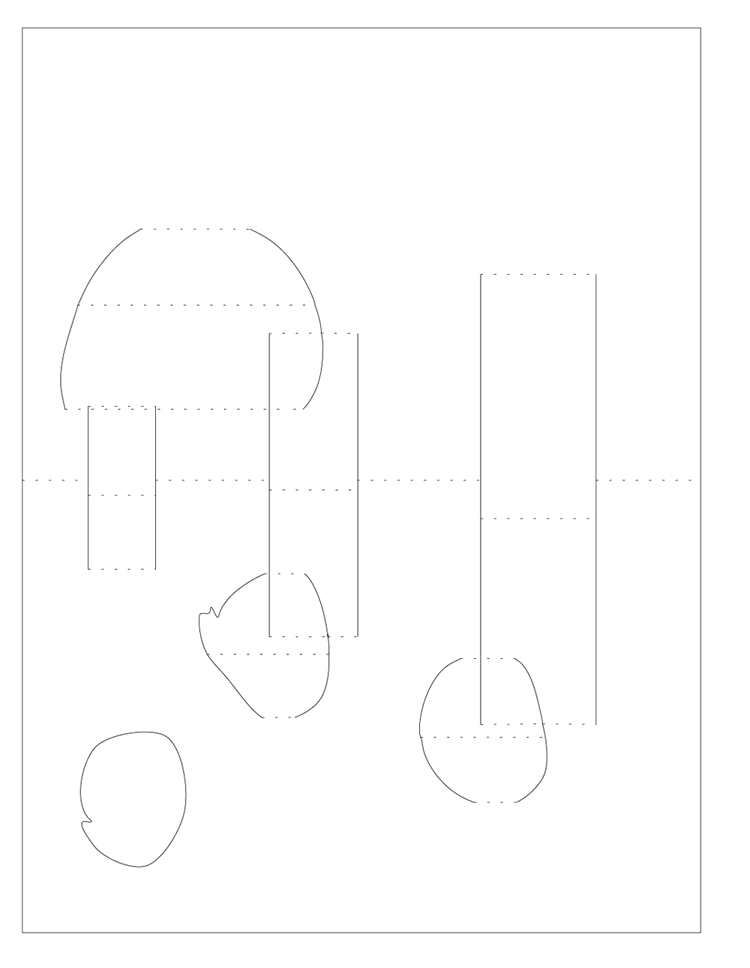
\includegraphics{figures/91_Appendix_DAX_Creations/overlapping_features.png}
\caption{An attempted sketch with overlapping features.}
\end{figure}

As we observed at the Digital Arts Exhibition\footnote{See section
  chapter \textbf{\textgreater{}\textgreater{}TODO}}, users often
attempt to draw features that overlap with existing features in the
sketch. To allow users to perform these kinds of operations as expected,
we allow for feature intersections.

Our intersection algorithm attempts to resolve overlapping features, by
occluding existing edges with the new feature and. The new feature is
drawn ``on top'' of existent features in the sketch. This is a complex
problem, and is only partly implemented\footnote{For example, we do not
  currently support intersections between all types of FoldFeature. In
  order to do feature-feature intersections in Foldlings, we transform
  all intersecting features into the same type, to simplify the process.
  At the current time, only freeform shapes an polygons are supported.}
due to the complexity involved in adding intersections to our system.
Currently, we display an error message if the intersected feature will
have any folds less than the minimum edge length after intersection. A
more complete implementation would analyze the resulting geometry for
potential problems.

\begin{algorithm}[H]
\ForEach{\textit{feature} in \textit{sketch}}{

\If{\textit{feature} intersects with current drawing feature}{

\ForEach{\textit{edge} in \textit{feature}}{

\textit{intercepts} $\leftarrow$ all points of intersection between \textit{feature} and current drawing feature

\If{\textit{intercepts} not nil}{

\textit{fragments} $\leftarrow$ \textit{edge} split by \textit{intercepts} 

\ForEach{\textit{fragment} in \textit{fragments}}{

\If{center of \textit{fragment} inside bounds of current drawing feature}{

remove \textit{fragment} from \textit{sketch} 

}

}

}

}

reassign \textit{fragments} as edges of \textit{feature}

}

}

recalculate planes for \textit{sketch}
\
\
\caption{Feature Intersections}
\end{algorithm}

\begin{figure}[htbp]
\centering
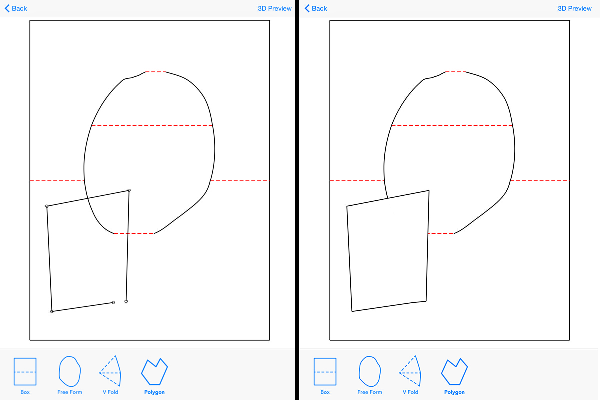
\includegraphics{figures/43_Tech_Intersections_Between_Features/featureIntBeforeAfter.pdf}
\caption{New polygon feature intersecting with an existing freeform
shape.}
\end{figure}
